
% v2-acmsmall-sample.tex, dated March 6 2012
% This is a sample file for ACM small trim journals
%
% Compilation using 'acmsmall.cls' - version 1.3 (March 2012), Aptara Inc.
% (c) 2010 Association for Computing Machinery (ACM)
%
% Questions/Suggestions/Feedback should be addressed to => "acmtexsupport@aptaracorp.com".
% Users can also go through the FAQs available on the journal's submission webpage.
%
% Steps to compile: latex, bibtex, latex latex
%
% For tracking purposes => this is v1.3 - March 2012
\documentclass[prodmode,acmtecs]{acmsmall} % Aptara syntax
\usepackage[spanish,polish]{babel}
\usepackage[T1]{fontenc}
\usepackage{fancyvrb}
\usepackage{graphicx,hyperref}
\newcommand\cutout[1]{}


\usepackage[table]{xcolor}
\usepackage[utf8]{inputenc}
\usepackage[parfill]{parskip}
\usepackage{tabulary}
\PassOptionsToPackage{hyphens}{url}
\usepackage{hyperref}    
\usepackage[capitalize]{cleveref}


% Metadata Information
% !!! TODO: SET THESE VALUES !!!
\acmVolume{0}
\acmNumber{0}
\acmArticle{CFP}
\acmYear{0}
\acmMonth{0}

\newcounter{colstart}
\setcounter{page}{4}

\RecustomVerbatimCommand{\VerbatimInput}{VerbatimInput}%
{
%fontsize=\footnotesize,
fontfamily=\rmdefault
}


\newcommand{\UnderscoreCommands}{%\do\verbatiminput%
\do\citeNP \do\citeA \do\citeANP \do\citeN \do\shortcite%
\do\shortciteNP \do\shortciteA \do\shortciteANP \do\shortciteN%
\do\citeyear \do\citeyearNP%
}

\usepackage[strings]{underscore}



% Document starts
\begin{document}


\setcounter{colstart}{\thepage}

\acmArticle{CFP}
\title{\huge\sc SIGLOG Monthly 221}
\author{DAVID PURSER\affil{Max Planck Institute for Software Systems, Saarbr\"ucken}
\vspace*{-2.6cm}\begin{flushright}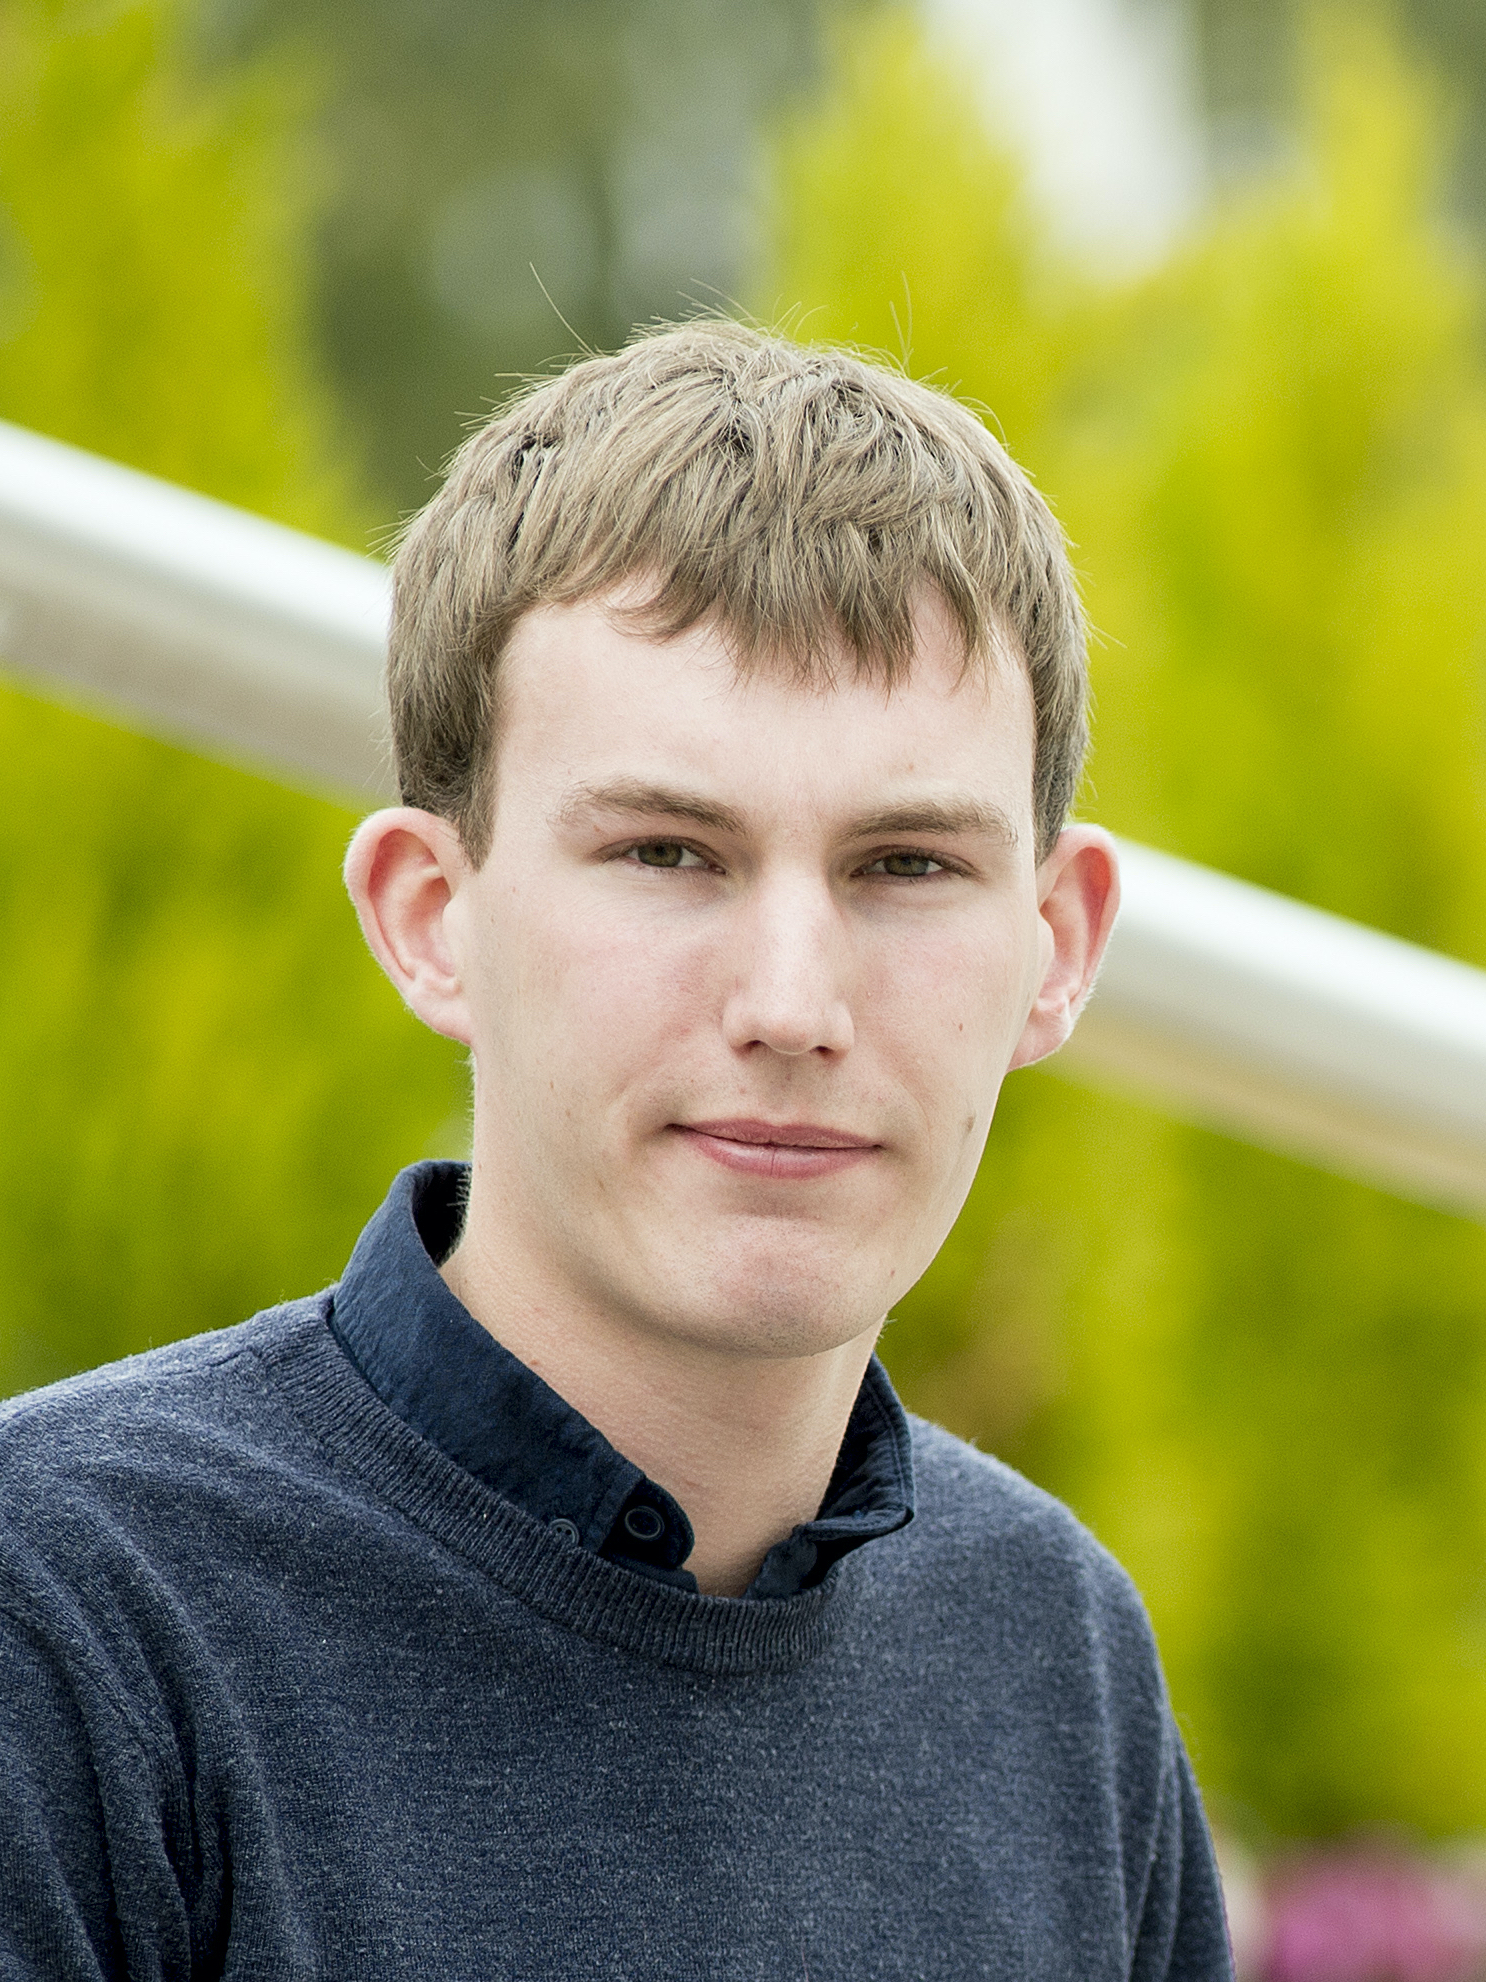
\includegraphics[width=30mm]{dp}\end{flushright}
}

\maketitlee

\href{https://lics.siglog.org/newsletters/}{Past Issues}
 - 
\href{https://lics.siglog.org/newsletters/inst.html}{How to submit an announcement}
\section{Table of Content}\begin{itemize}\item DEADLINES (\cref{deadlines}) 
 
\item ANNOUNCEMENTS 
 
\begin{itemize}\item TheoretiCS (\cref{TheoretiCS})
\item MOVEP 2022 (\cref{MOVEP2022})
\end{itemize} 
\item CALLS 
 
\begin{itemize}\item CPP 2022 (CALL FOR PARTICIPATION) (\cref{CPP2022})
\item IJCAR 2022 (CALL FOR PAPERS) (\cref{IJCAR2022})
\item ICGT 2022 (CALL FOR PAPERS) (\cref{ICGT2022})
\item FORMATS 2022 (CALL FOR PAPERS) (\cref{FORMATS2022})
\item ATVA 2022 (CALL FOR PAPERS) (\cref{ATVA2022})
\end{itemize} 
\end{itemize}\section{Deadlines}\label{deadlines}\rowcolors{1}{white}{gray!25}\begin{tabulary}{\linewidth}{LL}NFM 2022:  & Jan 03, 2022 (Abstract, EXTENDED), Jan 10, 2022 (Paper, EXTENDED) \\
CPP 2022:  & Jan 03, 2022 (Registration deadline) \\
CiE 2022:  & Jan 14, 2022 (Article registration, abstract), Jan 28, 2022 (Article) \\
LICS 2022:  & Jan 17, 2022 (Titles and Short Abstracts Due), Jan 21, 2022 (Full Papers Due) \\
CAV 2022:  & Jan 21, 2022 (Paper) \\
FSCD 2022:  & Jan 22, 2022 (Call for Locations), Feb 08, 2022 (Abstract), Feb 11, 2022 (Paper) \\
FoIKS 2022:  & Feb 04, 2022 (Abstract), Feb 11, 2022 (Paper) \\
IJCAR 2022:  & Feb 11, 2022 (Paper) \\
ICGT 2022:  & Feb 21, 2022 (Abstract), Feb 28, 2022 (Paper) \\
AiML 2022:  & Mar 07, 2022 (Abstracts for full papers), Mar 14, 2022 (Full papers), May 23, 2022 (Short presentations) \\
TYPES 2022 and CA20111:  & Mar 09, 2022 (2 page abstract) \\
FORMATS 2022:  & Apr 19, 2022 (Abstract), Apr 22, 2022 (Paper) \\
ATVA 2022:  & Apr 24, 2022 (Abstract), May 01, 2022 (Paper) \\
\end{tabulary}
\section{TheoretiCS: Launch of a new diamond open-access journal for TCS}\label{TheoretiCS}  \href{http://www.theoretics-journal.org}{http://www.theoretics-journal.org}\\ 
ANNOUNCEMENT 

\begin{itemize}\item  TheoretiCS is firmly rooted in the Theoretical Computer Science global community. It has involved an unprecedented level of cooperation of representatives of leading conferences from across the entire Theoretical Computer Science community. Its Advisory Board is composed of representatives of most of the main conferences in the field (currently APPROX, CCC, COLT, CONCUR, CSL, FOCS, FoSSaCS, FSCD, FSTTCS, ICALP, ICDT, ITCS, LICS, MFCS, PODC, SoCG, SODA, STACS, STOC, TCC) and of a few further ``members-at-large''. 
 
\item  The scope of TheoretiCS is the whole of Theoretical Computer Science, understood in an inclusive meaning. 
 
\item  The aim of this journal is to rapidly become a reference journal and to contribute to the unity of the Theoretical Computer Science global community. In particular, we will seek to publish only papers that make a very significant contribution to their respective fields, that strive to be accessible to a wider audience within theoretical computer science, and that are, generally, of a quality on par with the very best journals in the field. 
 
\item  TheoretiCS adheres to the principles of diamond open-access: there is no charge to read the journal, nor to publish in it. The copyright of the papers remains with the authors, under a Creative Commons license. 
 
\item  The inaugural Editors-in-Chief are Javier Esparza (TU München) and Uri Zwick (Tel Aviv U.).   See the website above for the entire Editorial Board and instructions for submission. 
 
\end{itemize}\section{MOVEP 2022: 15th Summer School on Modelling and Verification of Parallel Processes}\label{MOVEP2022}  Aalborg University, Aalborg, Denmark\\ 
  June 13 - 17, 2022\\ 
  \href{https://movep2022.cs.aau.dk/}{https://movep2022.cs.aau.dk/}\\ 
ANNOUNCEMENT 

\begin{itemize}\item  MOVEP is a five-day summer school on modelling and verification of infinite state systems. It aims to bring together researchers and students working in the fields of control and verification of concurrent and reactive systems. 
 
\item  MOVEP 2022 will consist of ten invited tutorials. In addition, there will be special sessions that allow PhD students to present their on-going research (each talk will last around 20 minutes). Extended abstracts (1-2 pages) of these presentations will be published in informal proceedings. 
 
\item  Confirmed Speakers 
 
\begin{itemize}\item  Anca Muscholl (LaBRI \& Université Bordeaux, France)
\item  Amaury Pouly (IRIF, France)
\item  Nir Piterman (Chalmers University of Technology, Sweden)
\item  Christel Baier (Technische Universität Dresden, Germany)
\item  Laura Kovacs (Vienna University of Technology, Austria)
\item  Wojcziech Czerwinski (University of Warsaw, Poland)
\item  Giovanni Bacci (Aalborg University, Denmark)
\item  Bartek Klin (Oxford University, United Kingdom) 
\item  Renaud Vilmart (LMF \& Inria)
\item  David Baelde (ENS Rennes \& IRISA)  
\end{itemize} 
\item  Registration will open in January 2022, abstract submission for the student session will be in early spring 2022. 
 
\end{itemize}\section{CPP 2022: Certified Programs and Proofs }\label{CPP2022}  \href{https://popl22.sigplan.org/home/CPP-2022}{https://popl22.sigplan.org/home/CPP-2022}\\ 
  Collocated with POPL \\ 
  17-18 January 2022\\ 
  Accepted papers: \href{https://popl22.sigplan.org/home/CPP-2022#event-overview}{https://popl22.sigplan.org/home/CPP-2022\#event-overview}\\ 
  Early registration deadline: 3 January 2022\\ 
  Registration: \href{https://popl22.sigplan.org/attending/registration}{https://popl22.sigplan.org/attending/registration}\\ 
  Accommodation: \href{https://popl22.sigplan.org/venue/POPL-2022-venue}{https://popl22.sigplan.org/venue/POPL-2022-venue}\\ 
CALL FOR PARTICIPATION 

\begin{itemize}\item  Certified Programs and Proofs (CPP) is an international conference on practical and theoretical topics in all areas that consider formal verification and certification as an essential paradigm for their work. CPP spans areas of computer science, mathematics, logic, and education. 
 
  CPP 2022 (\href{https://popl22.sigplan.org/home/CPP-2022}{https://popl22.sigplan.org/home/CPP-2022}) will be held on 17-18 January 2022 and will be co-located with POPL 2022. CPP 2022 is sponsored by ACM SIGPLAN, in cooperation with ACM SIGLOG, and supported by a diverse set of industrial sponsors. 
 
  Similarly to other events collocated with POPL 2022, CPP will take place as an in-person event at the Westin Philadelphia (99 South 17th Street at Liberty Place, 19103 Philadelphia), and will require attendees to provide proof of vaccination (details will be available soon). Authors who are unable to attend CPP in person will be able to present remotely. All talks will be recorded, and all recordings will be available either as a livestream or soon afterwards. 
 
\item  INVITED TALKS 
 
\begin{itemize}\item  June Andronick (UNSW Sydney). The seL4 verification: the art and craft of proof and the reality of commercial support
\item  Andrew W. Appel (Princeton). Coq’s vibrant ecosystem for verification engineering
\item  Cesar Munoz (Currently at AWS, Formerly at NASA, USA). Structural Embeddings Revisited
\end{itemize} 
\item  SUBSIDIZED STUDENT REGISTRATION 
 
  To facilitate in-person participation of undergraduate and graduate students who require financial assistance, CPP 2022 offers the opportunity to register at a special reduced rate, determined on a case-by-case basis, and implemented using a special-purpose registration code on POPL's registration website. Students wishing to apply for such support may do so by sending an email to the CPP conference co-chairs (Beringer and Krebbers, see below for their email) preferably by December 24, 2021, with a brief description of their situation. Notifications will be sent out at most one week later; hence, students who cannot be supported will still have the opportunity to register at the publicly available reduced rate, which is available until January 3rd. Applications arriving after December 24th will be considered only in exceptional cases. Students who already receive registration support for PLMW or are supported by SIGPLAN PAC are not eligible. 
 
  CPP's student support is made possible by our generous industrial supporters: \href{https://popl22.sigplan.org/home/CPP-2022}{https://popl22.sigplan.org/home/CPP-2022}  
 
\end{itemize}\section{IJCAR 2022: International Joint Conference on Automated Reasoning 2022}\label{IJCAR2022}  \href{https://easychair.org/smart-program/IJCAR2022/}{https://easychair.org/smart-program/IJCAR2022/}.\\ 
CALL FOR PAPERS 

\begin{itemize}\item  Important Dates 
 
\rowcolors{1}{white}{gray!25}\begin{tabulary}{\linewidth}{LL}Paper submission:  & Feb 11, 2022 \\
Start of authors response period:  & Apr 16, 2022 \\
End of authors response period:  & Apr 18, 2022 \\
Authors notification:  & Apr 25, 2022 \\
\end{tabulary}
 
\item  OVERVIEW 
 
  IJCAR is the premier international joint conference on all aspects of automated  reasoning. IJCAR 2022 is the 11th edition of IJCAR. It will be held in Haifa (Israel), during August 7-12, 2022, as part of FLoC 2022. IJCAR 2022 is the merger conference of the following leading events in automated reasoning: 
 
\begin{itemize}\item  CADE (Conference on Automated Deduction)
\item  FroCoS (Symposium on Frontiers of Combining Systems)
\item  TABLEAUX (Conference on Analytic Tableaux and Related Methods)
\end{itemize} 
\item  SUBMISSION GUIDELINES 
 
  IJCAR 2022 invites submissions related to all aspects of automated or interactive reasoning, including foundations, implementations, and applications. All papers must be original and not simultaneously submitted to another journal or conference. The following paper categories are welcome: 
 
\begin{itemize}\item  Regular papers describing solid new research results. They can be up to 16 pages long, including figures but excluding references and appendices. Where applicable, regular papers are supported by experimental validation. Submissions reporting on case studies in an industrial context are strongly invited as regular papers, and should describe details, weaknesses and strength in sufficient depth.
\item  System description papers describing implementations of systems, reporting on novel features and experiments with implemented systems. System description papers can be up to 7 pages long, including figures but excluding references and appendices. System description papers should also be supported by a link to the artifact/experimental evaluation available to the reviewers. Each of these papers should mention the phrase ``(system description)" beneath the title. Papers describing tools that have already been presented in other conferences before will be accepted only if significant and clear enhancements to the tool are reported and implemented.
\end{itemize} 
  Both types of papers must be formatted using the Springer LNCS styles and submitted in PDF via EasyChair: \href{https://easychair.org/conferences/?conf=ijcar2022}{https://easychair.org/conferences/?conf=ijcar2022} 
 
  Authors of accepted papers are required to ensure that at least one of them will present the paper at the conference. 
 
\item  LIST OF TOPICS  
 
  IJCAR 2022 topics include the following ones: 
 
\begin{itemize}\item  Logics of interest include: propositional, first-order, classical, equational, higher-order, non-classical, constructive, modal, temporal, many-valued, substructural, description, type theory.
\item  Methods of interest include: tableaux, sequent calculi, resolution, model- elimination, inverse method, paramodulation, term rewriting, induction, unification, constraint solving, decision procedures,model generation, model checking, semantic guidance, interactive theorem proving, logical frameworks, AI-related methods for deductive systems, proof presentation, automated theorem proving, combination of decision or proof procedures, SAT and SMT solving, integration of proof assistants with automated provers and other symbolic tools, etc.
\item  Applications of interest include: verification, formal methods, program analysis and synthesis, computer mathematics, declarative programming, deductive databases, knowledge representation, education, formalization of mathematics etc.
\end{itemize} 
\item  PUBLICATION 
 
  IJCAR 2022 proceedings will be published in the Springer LNCS series. Springer encourages authors to include their ORCIDs in their papers. 
 
\end{itemize}\section{ICGT 2022: 15th International Conference on Graph Transformation}\label{ICGT2022}  \href{https://icgt2022.gitlab.io/}{https://icgt2022.gitlab.io/}\\ 
  July 7-8, Nantes, France, co-located with STAF 2022\\ 
CALL FOR PAPERS 

\begin{itemize}\item  AIMS AND SCOPE 
 
  The use of graphs and graph-like structures as a formalism for specification and modelling is widespread in all areas of computer science as well as in many fields of computational research and engineering. Relevant examples include software architectures, pointer structures, state space and control/data flow graphs, UML and other domain-specific models, network layouts, topologies of cyber-physical environments, quantum computing and molecular structures. Often, these graphs undergo dynamic change, ranging from reconfiguration and evolution to various kinds of behaviour, all of which may be captured by rule-based graph manipulation. Thus, graphs and graph transformation form a fundamental universal modelling paradigm that serves as a means for formal reasoning and analysis, ranging from the verification of certain properties of interest to the discovery of fundamentally new insights. 
 
  The International Conference on Graph Transformation aims at fostering exchange and collaboration of researchers from different backgrounds working with graphs and graph transformation, either in contributing to their theoretical foundations or by applying established formalisms to classical or novel areas. The conference not only serves as a well-established scientific publication outlet, but also as a platform to boost inter- and intra-disciplinary research and to leeway for new ideas. 
 
  The 15th International Conference on Graph Transformation (ICGT 2022) will be held in Nantes, France, as part of STAF 2022 (Software Technologies: Applications and Foundations). The conference takes place under the auspices of EATCS and IFIP WG 1.3. Proceedings will be published by Springer in the Lecture Notes in Computer Science (LNCS) series. 
 
\item  IMPORTANT DATES (AoE) 
 
\rowcolors{1}{white}{gray!25}\begin{tabulary}{\linewidth}{LL}Abstract submission:  & Feb 21, 2022 \\
Paper submission:  & Feb 28, 2022 \\
Notification:  & Apr 18, 2022 \\
Camera-ready:  & May 09, 2022 \\
Conference:  & Jul 7-8, 2022 \\
\end{tabulary}
 
\item  TOPICS OF INTEREST 
 
  In order to foster a lively exchange of perspectives on the subject of the conference, the programme committee of ICGT 2022 encourages all kinds of contributions related to graphs and graph transformation, either from a theoretical point of view or a practical one. 
 
  Topics of interest include, but are not limited to the following subjects: 
 
\begin{itemize}\item  General models of graph transformation (e.g. adhesive categories and hyperedge replacement systems); Analysis and verification of graph transformation systems; Graph theoretical properties of graph languages; Automata on graphs and parsing of graph languages; Logical aspects of graph transformation; Computational models based on graphs; Structuring and modularization of graph transformation; Hierarchical graphs and decomposition of graphs; Parallel, concurrent, and distributed graph transformation; Term graph and string diagram rewriting; Petri nets and other models of concurrency; Business process models and notations; Bigraphs and bigraphical reactive systems; Graph databases and graph queries; Model-driven development and model transformation; Model checking, program analysis and verification, simulation and animation; Syntax, semantics and implementation of programming languages, including domain-specific and visual languages; Graph transformation languages and tool support; Efficient algorithms (e.g. pattern matching, graph traversal, network analysis); Applications and case studies in software engineering (e.g. software architectures, refactoring, access control, and service-orientation); Applications to computing paradigms (e.g. bio-inspired, quantum, ubiquitous, and visual); Graph transformation and artificial intelligence (e.g., AI for graph transformations, applying graph transformations in AI engineering and search-based software engineering)
\end{itemize} 
\item  SPECIAL INTEREST TOPIC OF ICGT 2022: EXECUTABLE APPLIED CATEGORY THEORY 
 
  A special focus of this conference will consist of new approaches to formalizing the knowledge in the research field of graph transformation theory via proof assistants such as Coq. Referring to the homepage of the GReTA-ExACT workgroup for further information \href{https://www.irif.fr/~greta/gretaexact/}{https://www.irif.fr/~greta/gretaexact/}, a long-term goal of this kind of approach will consist in establishing a Coq-enriched wiki for our research field akin to the nLab. This platform will serve as a sustainable mechanism for curating applied and mathematical knowledge in graph transformation research, and eventually as a research tool in its own right, notably through the provision of interactive database-supported proof construction. Another avenue of research will concern executable applied category theory (ExACT), i.e., code extraction from formalized categorical structures, with the perspective of curating a database of correct-by-construction reference prototype algorithms for various forms of graph transformation semantics and graph-like data structures. To introduce the initiative and facilitate the broad involvement of the ICGT community and collect feedback from participants regarding the scope and format of such a wiki project, a peer-reviewed brainstorming session is planned as one of the events at the conference. 
 
\item  SUBMISSION GUIDELINES 
 
  Springer’s LNCS format via EasyChair \href{https://easychair.org/conferences/?conf=icgt2022}{https://easychair.org/conferences/?conf=icgt2022} using . For regular and tool demonstration papers, simultaneous submission to other conferences with proceedings or submission of material that has already been published elsewhere is not allowed. At least one author for each accepted paper must register before the early registration deadline and present the paper during the conference. 
 
  Papers are solicited in three categories: 
 
\begin{itemize}\item  Regular papers (max 16 pages inc references) describe innovative contributions and are evaluated with respect to their originality, significance, and technical soundness. We also solicit case studies describing applications of graph transformation in any application domain. Additional material intended for reviewers but not for publication in the final version may be included in a clearly marked appendix.
\item  Tool presentation papers (max 8 pages inc references) demonstrate the main features and functionality of graph-based tools. A tool presentation paper may have an appendix with a detailed demo description (up to 4 pages), which will be reviewed but not included in the proceedings.
\item  New ideas papers (max 2 pages inc references) report on relevant contributions to the theory or applications of graph transformation, which may have been published (or accepted for publication) in a peer-reviewed conference other than ICGT, as a book chapter or journal article since 2018. Papers in this category will be selected for presentation at the conference according to their relevance to the graph transformation community, and they will be considered for the special issues. Submissions will consist of a 2-page abstract. In case of extended abstracts of published papers, the submission must refer to the published paper and include the original paper in PDF.
\end{itemize} 
\item  SPECIAL ISSUE 
 
  Authors of the best papers at the conference will be invited to prepare and submit extended journal versions to be considered for publication in a special issue after an independent round of peer review (details TBA). 
 
\item  CONTACT 
 
  All questions about submissions should be emailed to icgt2022.info@gmail.com. 
 
\end{itemize}\section{FORMATS 2022: 20th International Conference on Formal Modeling and Analysis of Timed Systems}\label{FORMATS2022}  \href{https://conferences.ncl.ac.uk/formats2022/}{https://conferences.ncl.ac.uk/formats2022/}\\ 
  12-17 September 2022, Warsaw, Poland co-located with CONCUR, FMICS and QEST as part of CONFEST 2022\\ 
CALL FOR PAPERS 

\begin{itemize}\item  SCOPE and TOPICS 
 
  FORMATS (International Conference on Formal Modeling and Analysis of Timed Systems) is an annual conference which aims to promote the study of fundamental and practical aspects of timed systems, and to bring together researchers from different disciplines that share interests in the modelling, design and analysis of timed computational systems. The conference aims to attract researchers interested in real-time issues in hardware design, performance analysis, real-time software, scheduling, semantics and verification of real-timed, hybrid and probabilistic systems. 
 
\item  TOPICS 
 
  Typical topics include (but are not limited to): 
 
\begin{itemize}\item  Foundations and Semantics: Theoretical foundations of timed systems, languages and models (e.g., timed automata, timed Petri nets, hybrid automata, timed process algebra, max-plus algebra, probabilistic models).
\item  Methods and Tools: Techniques, algorithms, data structures, and software tools for analyzing timed systems and resolving temporal constraints (e.g., scheduling, worst-case execution time analysis,optimization, model checking, testing, constraint solving).
\item  Applications: Adaptation and specialization of timing technology in application domains in which timing plays an important role (e.g., real-time software, hardware circuits, scheduling in manufacturing and telecommunication, robotics).
\end{itemize} 
  New for this year, FORMATS will incorporate a special track on: 
 
\begin{itemize}\item  Learning-based and data-driven systems: We particularly encourage papers that exploit synergies between the formal analysis of timed systems and data-driven techniques (such as reinforcement learning or deep learning), or which target application domains where learning is important (such as robotics or autonomous systems).
\end{itemize} 
\item  PAPER SUBMISSION 
 
  FORMATS 2022 solicits high-quality papers reporting research results, experience reports and/or tools related to the topics mentioned above. Submitted papers must contain original, unpublished contributions, not submitted for publication elsewhere. The papers should be submitted electronically in PDF, following the Springer LNCS style guidelines. Two categories of papers are invited: 
 
\begin{itemize}\item  Regular papers, which should not exceed 15 pages in length
\item  Short papers, which should not exceed 7 pages in length
\end{itemize} 
  Both page limits exclude references, which are not limited in length. If necessary, the paper may be supplemented with a clearly marked appendix, which will be reviewed at the discretion of the program committee. Each paper will undergo a thorough review process. Papers should be submitted electronically via the EasyChair online submission system: \href{https://easychair.org/conferences/?conf=formats2022}{https://easychair.org/conferences/?conf=formats2022}  
 
\item  ARTIFACT EVALUATION 
 
  This year, FORMATS is encouraging authors to submit artifacts where appropriate, for example to demonstrate how to reproduce experimental data in a research paper or to examine the usability and applicability of a software tool. Artifacts will be submitted and evaluated only for papers accepted for publication. These will be evaluated by the Artifact Evaluation Committee and those that are accepted will receive a repeatability badge to be displayed on the first page of the published version. 
 
\item  PUBLICATION AND BEST PAPER AWARD 
 
  The proceedings of FORMATS 2022 will be published by Springer in the Lecture Notes in Computer Science series. The best paper of the conference will be awarded the Oded Maler Award in Timed Systems. 
 
\item  IMPORTANT DATES 
 
\rowcolors{1}{white}{gray!25}\begin{tabulary}{\linewidth}{LL}Abstract submission:  & Apr 19, 2022 \\
Paper submission:  & Apr 22, 2022 \\
Acceptance notification:  & Jun 17, 2022 \\
Artifact submission deadline:  & Jun 24, 2022 \\
Camera-ready copy deadline:  & Jul 15, 2022 \\
Conference:  & September 12-17, 2022 \\
\end{tabulary}
 
  CONFEST 2022, which includes FORMATS 2022, is currently planned as a physical, in-person event with support for remote presence for speakers and participants. Depending on the pandemic situation, a decision whether to cancel the physical component of CONFEST or not will be made by the end of June 2022. 
 
\item  CONTACT 
 
  For any questions, feel free to contact the program chairs Sergiy Bogomolov (sergiy.bogomolov@ncl.ac.uk) and David Parker d.a.parker@cs.bham.ac.uk). 
 
\end{itemize}\section{ATVA 2022: THE 20TH INTERNATIONAL SYMPOSIUM ON AUTOMATED TECHNOLOGY FOR VERIFICATION AND ANALYSIS }\label{ATVA2022}  October 25-28, 2022, Beijing, China. \\ 
  If the pandemic means that travelling is still an issue in October, we might change the plan and host the conference online.\\ 
  \href{https://atva-conference.org/2022/}{https://atva-conference.org/2022/}\\ 
CALL FOR PAPERS 

\begin{itemize}\item  ATVA 2022 is the 20th in a series of symposia aimed at bringing together academics, industrial researchers and practitioners in the area of theoretical and practical aspects of automated analysis, synthesis, and verification of hardware, software, and machine learning (ML) systems.  
 
\item  IMPORTANT DATES  (AOE) 
 
\rowcolors{1}{white}{gray!25}\begin{tabulary}{\linewidth}{LL}Abstract submission:  & Apr 24, 2022 \\
Paper submission:  & May 01, 2022 \\
Notification:  & Jun 17, 2022 \\
Camera-ready:  & Jul 15, 2022 \\
Conference:  & Oct 25-28, 2022 \\
\end{tabulary}
 
\item  ATVA solicits high-quality submissions in the following suggestive list of topics: 
 
\begin{itemize}\item  Formalisms for modeling hardware, software and cyber-physical systems
\item  Specifications and correctness criteria for programs and systems
\item  Decision procedures and solvers for verification and synthesis
\item  Deductive, algorithmic, compositional, and abstraction/refinement techniques for analysis and verification
\item  Program analysis and software verification
\item  Analysis and verification of hardware circuits and systems-on-chip 
\item  Analysis and verification of parallel and concurrent systems
\item  Analysis of probabilistic and cyber-physical systems
\item  Analysis and verification of machine learning algorithms and systems
\item  Formal models and methods for security and privacy
\item  Formal models and methods for biological systems
\item  Testing and runtime analysis based on verification technology
\item  Synthesis for hardware and software systems
\item  Applications and case studies
\item  Verification in industrial practice
\end{itemize} 
\end{itemize}


To the \href{http://siglog.org/}{SIGLOG} or \href{https://lics.siglog.org}{LICS} website\end{document}